
  
\documentclass{exam}
\usepackage[utf8]{inputenc}
\usepackage{upgreek}
\usepackage[margin=1in]{geometry}
\usepackage{amsmath,amssymb}
\usepackage{multicol}
\usepackage{stmaryrd}
\usepackage{graphicx}
\usepackage{caption}
\usepackage{tikz}
\usepackage{dsfont}
\usepackage{enumitem}
\usepackage{hyperref}
\usepackage{float}
\usetikzlibrary{matrix}
\newcommand\tab[1][1cm]{\hspace*{#1}}
\pagestyle{head}
\firstpageheader{}{}{}
\runningheader{\examnum}{\class}{\name}
\runningheadrule
\newcommand{\class}{Fundamentos de bases de datos}
\newcommand{\term}{Facultad de Ciencias UNAM}
\newcommand{\examnum}{Practica 08}
\newcommand{\examdate}{12/05/2022}
\newcommand{\name}{Jurassic Team}
\begin{document}

\noindent
\begin{tabular*}{\textwidth}{l @{\extracolsep{\fill}} r @{\extracolsep{6pt}} l}
\textbf{\class} & \textbf{\term}\\
\textbf{\examnum} & \textbf{\name}\\
\textbf{\examdate}
\end{tabular*}\\
\rule[2ex]{\textwidth}{2pt}

\section*{Herramientas utilizadas}

	Para la elaboración de el archivo \texttt{DML.sql} se utilizaron dos herramientas, mockaroo y un convertidor CSV a SQL.
	
	\begin{itemize}
		\item \textbf{Mockaroo}: Esta es una herramienta profesional utilizada para generar datos de prueba en base a un esquema definido por los usuarios. El uso de la herramienta es simple, primero se define el nombre de la tabla, luego de las columnas y finalmente el tipo de dato que lleva cada columna. Adicionalmente es posible agregar validaciones y/o funciones sobre los datos generados para obtener datos más específicos. Una vez que se define el esquema podemos validar que los datos generados tengan la estructura deseada dando click en \textbf{PREVIEW}. Si todo esta en orden generamos los datos en un archivo CSV. Aunque es posible generar datos en SQL directamente decidimos usar CSV para todos ya que de esta manera podemos conservar la integridad referencial entre nuestras tablas.
		
		\begin{figure}[h!]
			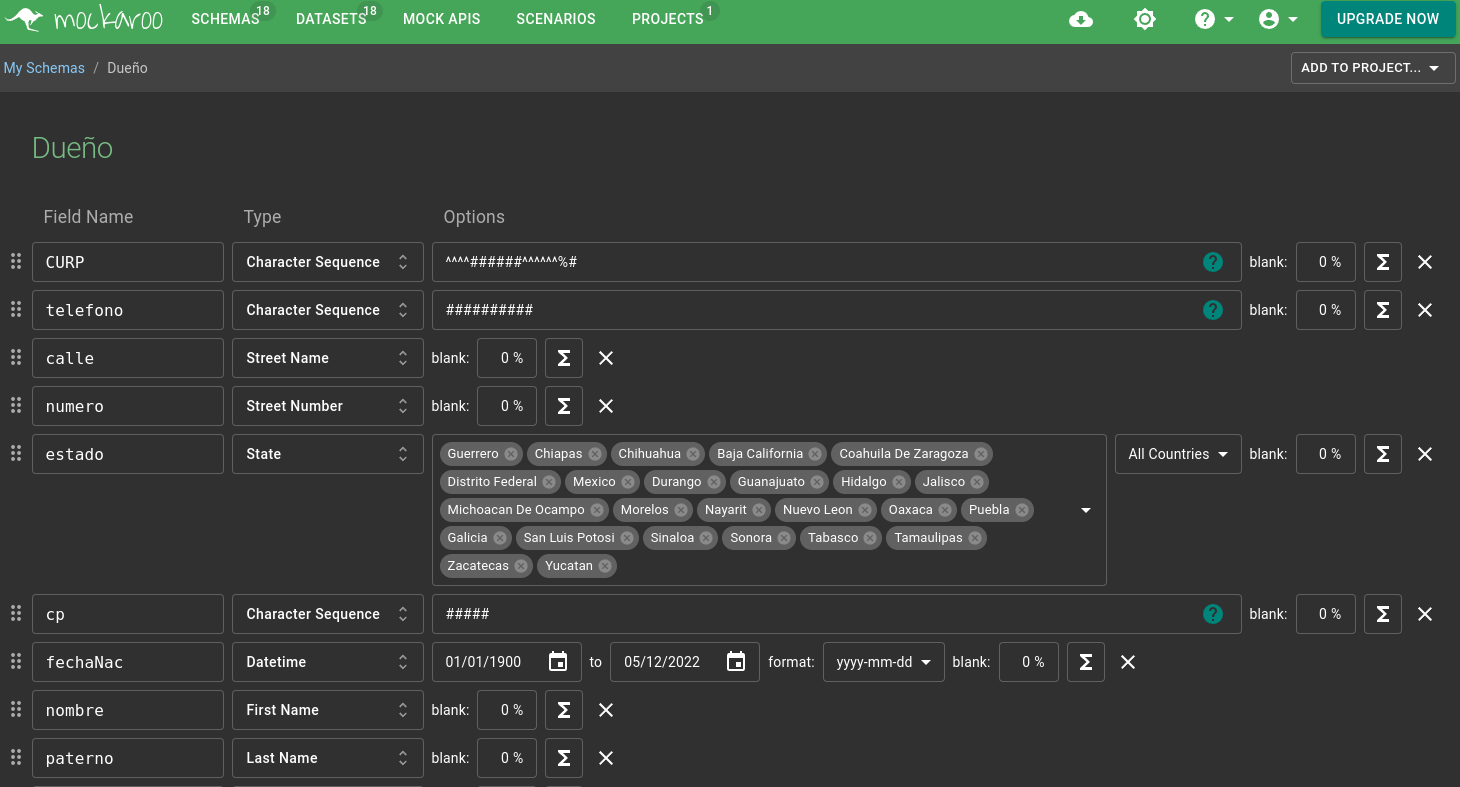
\includegraphics[scale=0.3]{mockaroo1.png}
			\centering
		\end{figure}		
		
		\begin{figure}[h!]
			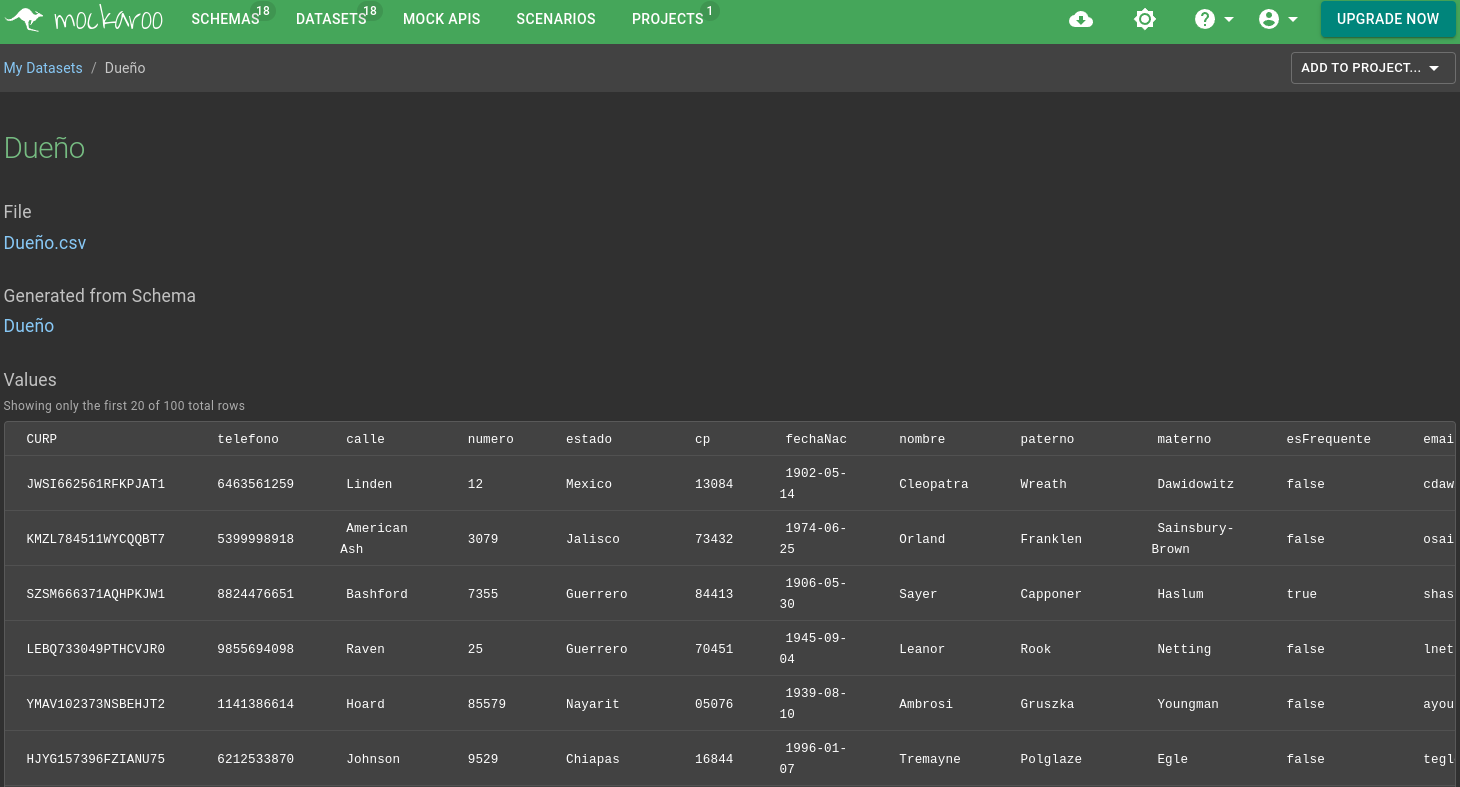
\includegraphics[scale=0.3]{mockaroo2.png}
			\centering
		\end{figure}	
		
		\pagebreak		
		
		\item \textbf{CSV2SQL}: Una pagina web hecha para convertir un archivo CSV en consultas INSERT de SQL. Para usarla simplemente cargamos los archivos CSV generados con mockaroo. Después validamos que los tipos de dato sean correctos y corregir si es necesario (como cambiar de tipo INT a VARCHAR el numero de teléfono). Generamos los archivos y esto da una lista de ordenes en lenguaje SQL simplemente copiamos/pegamos en \texttt{DML.txt} y terminamos
		
		\begin{figure}[h!]
			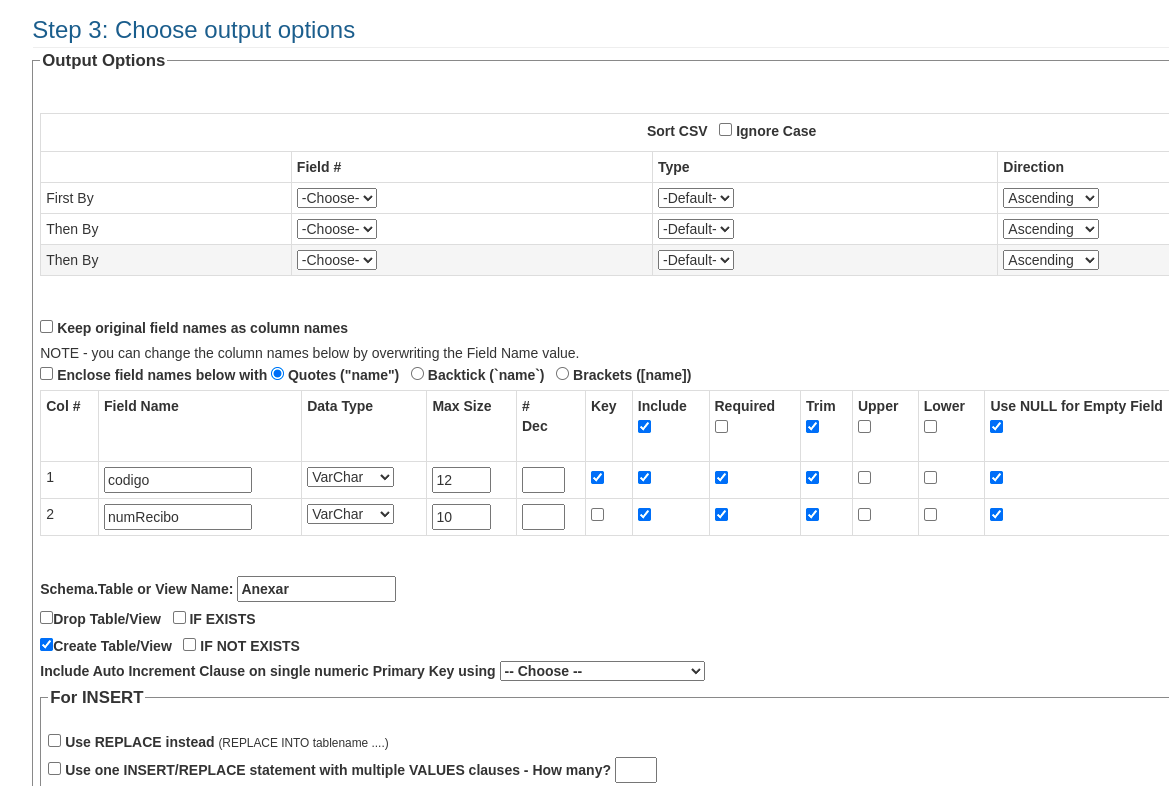
\includegraphics[scale=0.5]{csv2sql.png}
			\centering
		\end{figure}			
		
	\end{itemize}

\end{document}
